\label{latencies}
\section{Measurement of synaptic delay}
Stimfit is frequently used to measure the \keyindex{synapticdelay}{synaptic delay}{synaptic delay}delay between a presynaptic signal and a postsynaptic response. Classically, this synaptic delay or \index{latency}latency is defined as ``the time interval between peak of inward current through the presynaptic membrane and commencement of inward current through the postsynaptic membrane'' \cite{Katz65}. Neglecting cable properties of neurons for a while, the maximal inward current during an action potential is expected to flow at the time of maximal slope during the rising phase \cite{Jack83}, since
\begin{align*}
  &I_\text{m}=I_\text{cap}+I_\text{ionic}=C_\text{m}\frac{\text{d}V_\text{m}}{\text{d}t}+I_\text{ionic}=0\text{,~and~hence}\\
  &I_\text{ionic}=-I_\text{cap}=-C_\text{m}\frac{\text{d}V_\text{m}}{\text{d}t}
\end{align*}
The commencement \keyindex{foot}{foot}{foot}(sometimes called ``foot'') of the postsynaptic current can robustly be estimated from the extrapolated intersection of the baseline with a line through the two points of time when the current is 20 and 80\% of the peak current (\citetext{Jonas93,Bartos01}; Fig. \ref{epscfoot}).
  \begin{myfigure}[htb]
    \begin{center}
      \input{img/foot}
    \end{center}
    \caption{Foot of an EPSC (red circle), estimated from the extrapolated intersection of the baseline with a line through the two points of time when the current is 20 and 80\% of the peak current (black open circles).}
    \label{epscfoot}
  \end{myfigure}

Although the method described above yields reliable results when both the pre- and the postsynaptic whole-cell recording show little noise and few artefacts, it may sometimes be favourable to use other estimates for the pre- and postsynaptic signals, for example when extracellular stimulation was used or when there are a lot of failures in the postsynaptic response. The following sections will explain how this is done in practice.

\section{Trace alignment}
It may sometimes be useful to \keyindex{tracealignment}{traces!alignment}{trace alignment}align traces before measuring the latency, either for visualisation purposes or to create an average without temporal jitter. Although an aligned average can be created using a toolbar button, the recommended way to align traces is to use the Python shell. \smallskip \\
\pycommand{\textbf{align\_selected(alignment, active=False)}}\pyindex{alignselected}{align\_selected}\\
This function aligns the selected traces to a point that is determined by the user-supplied function \pycommand{alignment} and then shows the aligned traces in a new window. The \pycommand{alignment} function is applied to the active channel if \pycommand{active=True} or to the inactive channel if \pycommand{active=False}. The alignment function has to return an index within a trace, and it should adhere to the general form \pycommand{index(active)}, where \pycommand{active} is a boolean indicating whether the active or the inactive channel should be used. The most common alignment functions are built into the program: \smallskip \\
\pycommand{\textbf{maxrise\_index(active)}}\pyindex{maxriseindex}{maxrise\_index}\\
\noindent returns the zero-based index of the maximal slope of rise in units of sampling points (see Fig. \ref{overview}), interpolated between adjacent sampling points, or a negative value upon failure.\smallskip\\
\pycommand{\textbf{peak\_index(active)}}\pyindex{peakindex}{peak\_index}\\
\noindent returns the zero-based index of the peak value in units of sampling points (see Fig. \ref{overview}), or a negative value upon failure. The return value may be interpolated if a moving average is used for the peak calculation (see p. \pageref{peakmovingaverage}).\smallskip\\
\pycommand{\textbf{foot\_index(active)}}\pyindex{footindex}{foot\_index}\\
\noindent returns the zero-based index of the foot of an event, as described on p. \pageref{foot} and in Fig. \ref{epscfoot}, or a negative value upon failure.\smallskip\\
\pycommand{\textbf{t50left\_index(active)}}\pyindex{t50leftindex}{t50left\_index}\\
\noindent returns the zero-based index of the left half-maximal amplitude in units of sampling points (see Fig. \ref{overview}), or a negative value upon failure. The return value will be interpolated between sampling points.\smallskip\\
\pycommand{\textbf{t50right\_index(active)}}\pyindex{t50rightindex}{t50right\_index}\\
\noindent  returns the zero-based index of the right half-maximal amplitude in units of sampling points (see Fig. \ref{overview}), or a negative value upon failure. The return value will be interpolated between sampling points.\smallskip\\
Listing \ref{alignall} shows a function that can be used to align all traces within a file to the maximal slope of rise in the inactive channel:
\begin{listing}
\lstset{numbers=left}
\begin{lstlisting}
# import the stimfit core module:
import stf

def align_maxrise():
    """Aligns all traces to the maximal slope of rise 
    of the inactive channel. Baseline and peak cursors
    have to be set appropriately before using this
    function.
    
    Return value:
    True upon success, False otherwise."""
    
    stf.select_all()
    
    # check whether there is an inactive channel at all:
    if ( stf.maxrise_index( False ) < 0 ):
        print "File not open, or no second channel; \
               aborting now"
        return False
        
    stf.align_selected( stf.maxrise_index, False )
    return True

\end{lstlisting}
\lstset{numbers=none}
  \caption {
    \pycommand{align\_maxrise}
  }
  \label{alignall}
\end{listing}

\section{Setting the latency cursors}
The \keyindex{latencycursors}{latency!cursors}{latency cursors}latency cursors (plottes as dotted vertical blue lines) can either be set automatically to some predefined points within a trace, or manually using the mouse buttons. The predefined points can be chosen from the menu: ``Edit''$\rightarrow$``Measure latency from...'' and ``Edit''$\rightarrow$``Measure latency to...''. The ``beginning'' of an event refers to the foot as explained above (Fig. \ref{epscfoot}). If ``Manually'' is selected, the left and right mouse buttons can be used to set the first and second latency cursors while the latency mode is activated. To switch to the latency mode, you can either click the corresponding button in the toolbar (Fig. \ref{latencybutton}) or press \keybox{L}.
  \begin{myfigure}[ht]
    \begin{center}
      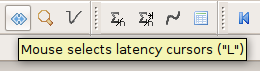
\includegraphics[scale = 0.5]{./img/latency.eps}
    \end{center}
    \caption{Activate latency mode.}
    \label{latencybutton}
  \end{myfigure}
  
To confirm your latency cursor settings and measure latencies, you can either press \keybox{Enter} or call \pycommand{measure()} from the shell (see p. \pageref{measure}). The latency, i.e. the time interval between the first and the second latency cursor, will be shown in the results table as long as you activated this value (see p. \pageref{resultstable}). The latency will be indicated as a double-headed arrow connecting the two latency cursors (Fig. \ref{latencytraces}).
  \begin{myfigure}[ht]
    \begin{center}
      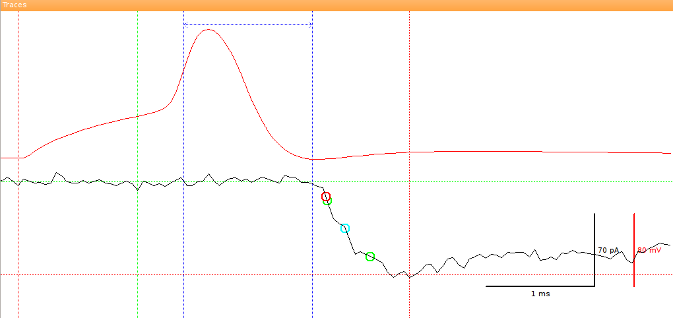
\includegraphics[scale = 0.4]{./img/latencytraces.eps}
    \end{center}
    \caption{The latency between the maximal slope of rise of an action potential (red) and the foot of an EPSC (black) is indicated by a horizontal double-headed arrow.}
    \label{latencytraces}
  \end{myfigure}
